\subsection{SharePoint}
\label{app:SharePoint}

\begin{figure}[htb]
    \centering
    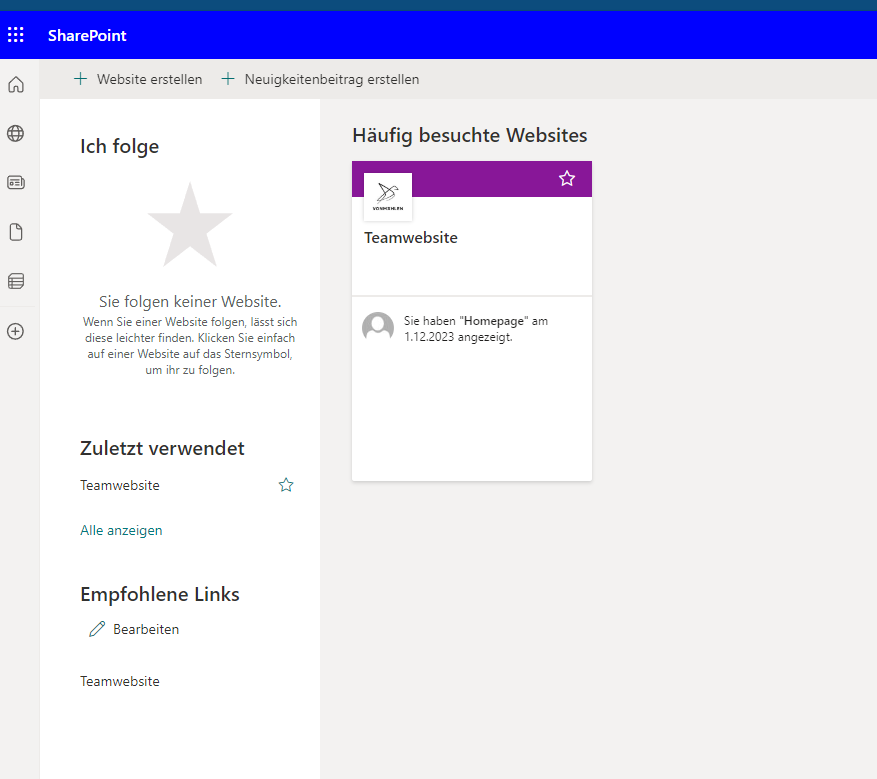
\includegraphics[width=0.6\textwidth]{01SharePoint Webseite erstellen.PNG}
    \caption{SharePoint Webseite erstellen}
    \label{fig:SharePointWebseiteErstellen}
\end{figure}

\begin{figure}[htb]
    \centering
    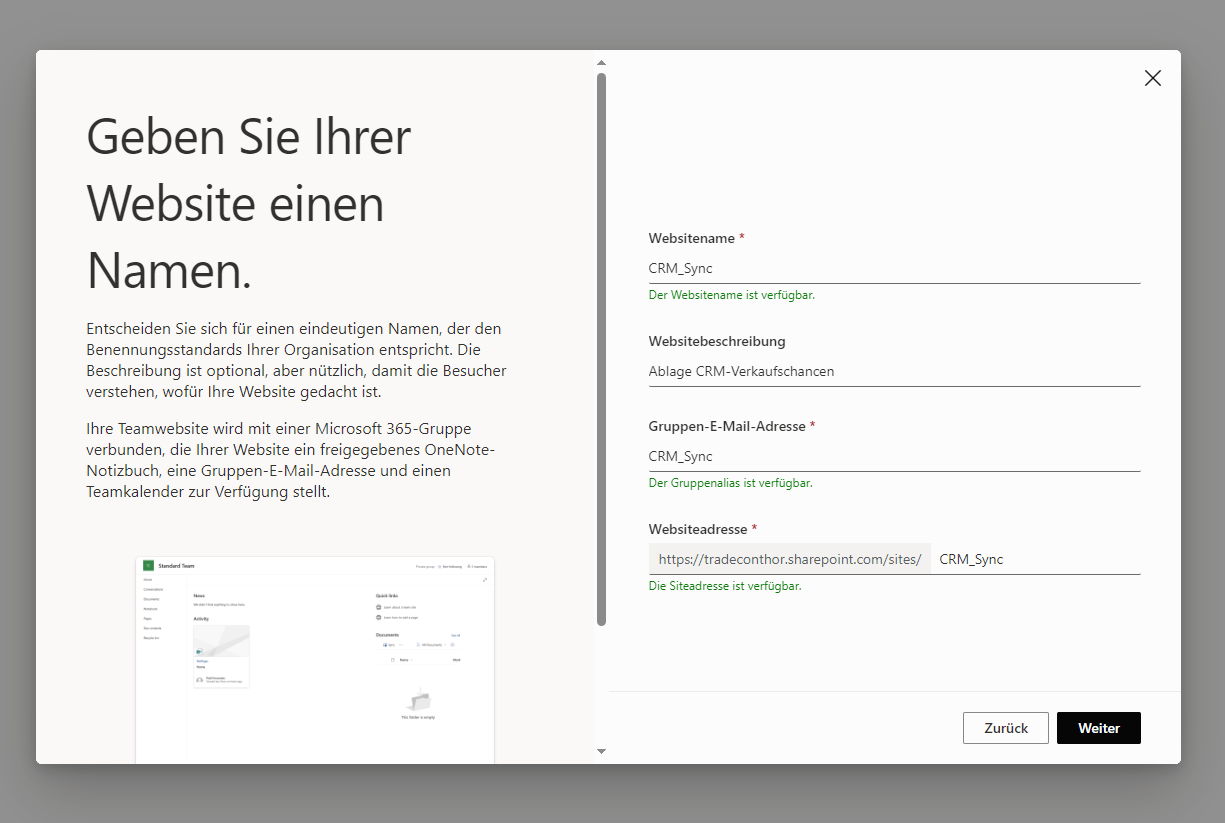
\includegraphics[width=0.6\textwidth]{02SharePoint Webseite CRM_Sync.PNG}
    \caption{Informationen zur SharePoint Webseite}
    \label{fig:SharePointWebseiteCRMSync}
\end{figure}

\begin{figure}[htb]
    \centering
    \includegraphics[width=0.4\textwidth]{14Mitglieder hinzufügen SharePoint.PNG}
    \caption{Hinzufügen der Mitglieder}
    \label{fig:MitgliederHinzufuegenSharePoint}
\end{figure}

\begin{figure}[htb]
    \centering
    \includegraphics[width=0.6\textwidth]{16Dokumentenbibliothek auswählen.PNG}
    \caption{Dokumentenbibliothek auswählen}
    \label{fig:DokumentenbibliothekAuswaehlen}
\end{figure}

\begin{figure}[htb]
    \centering
    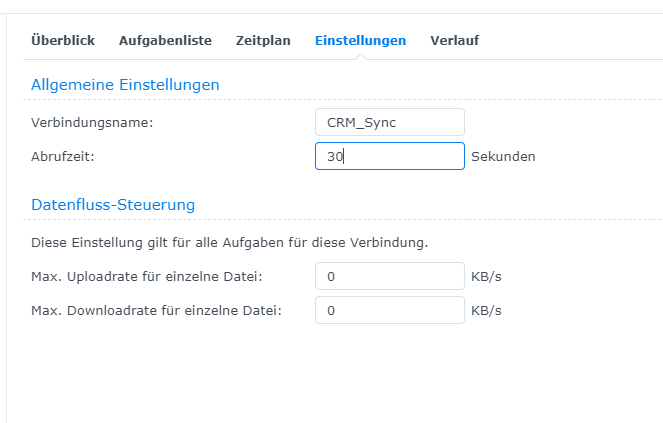
\includegraphics[width=0.6\textwidth]{19ZeitenSync.PNG}
    \caption{Zeiten einstellen zur Synchronisation}
    \label{fig:ZeitenSync}
\end{figure}
\clearpage
